%! Author = yessense
%! Date = 04.02.2022

\documentclass{article}
\usepackage[utf8]{inputenc}
\usepackage{graphicx}
\usepackage{hyperref}
\usepackage{wasysym}
\usepackage{amsfonts}
\usepackage{booktabs}
%\usepackage{siunitx}
\title{dSprites VSA}
\author{ }
\date{ }

\begin{document}

    \maketitle


    \section{Introduction}

    The goal of this work is to get a hidden disentanglement representation
    of the scene, such that we can, by performing certain operations on it,
    get predictable changes in the scene. That is, we move from manipulating
    the objects in the scene (pixels) to manipulating their hidden representations.


    \section{Datasets}
    The task consists of three consecutive steps for each of
    which a different dataset was created. These datasets are based on
    the dSprites dataset \autoref{fig:dsprites}.
    dSprites is a dataset of 2D shapes procedurally generated
    from 6 ground truth independent latent factors \autoref{tab:features}


    \begin{figure}[ht]
        \centering
        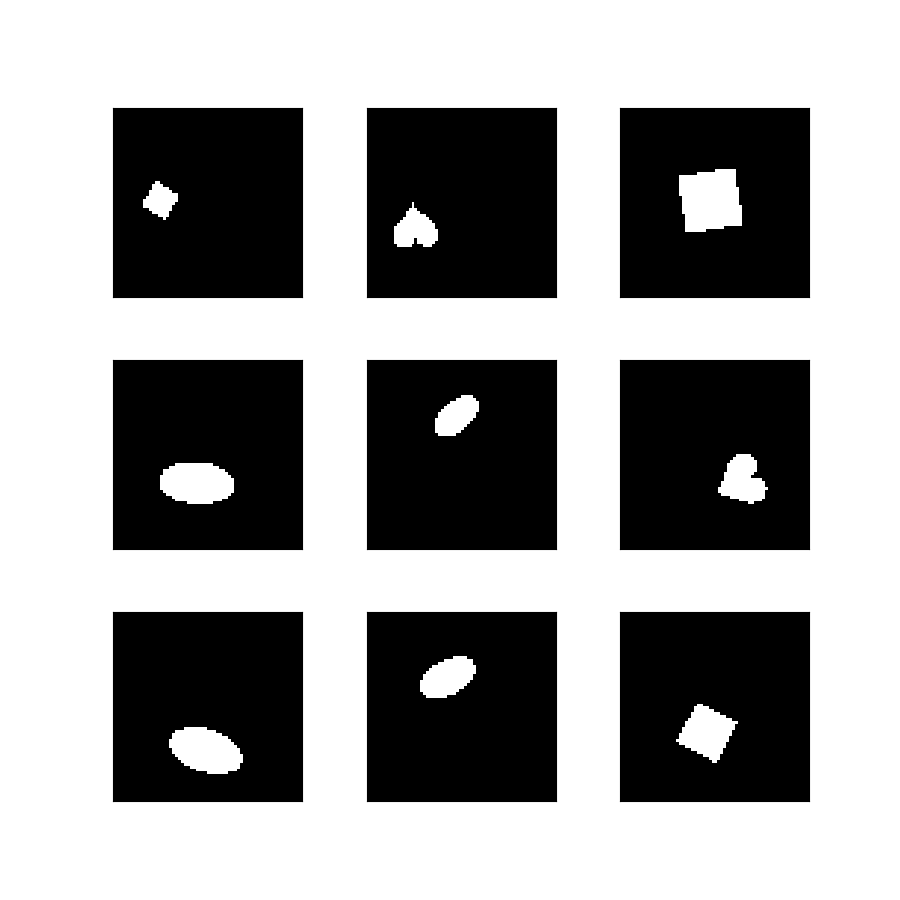
\includegraphics[width=0.3\textwidth]{img/datasets/dsprites}
        \caption{Example of images from dSprites dataset}
        \label{fig:dsprites}
    \end{figure}

    \begin{table}[ht]
        \centering
        \caption{List of features}
        \label{tab:features}
        \begin{tabular}[t]{ll}
            \hline
            Feature     & Distribution                         \\
            \hline
            Shape       & square, ellipse, heart               \\
            Scale       & 6 values linearly spaced in [0.5, 1] \\
            Orientation & 40 values in [0, 2 pi]               \\
            Position X  & 32 values in [0, 1]                  \\
            Position Y  & 32 values in [0, 1]                  \\
            \hline
        \end{tabular}
    \end{table}

    \subsection{Paired-dSprites dataset}

    The purpose of creating this dataset is to make it possible to easily
    obtain paired images that differ in a single feature. This is possible
    due to the fact that in the original dataset the images are arranged in
    an orderly manner.
    An example of pairwise images in a dataset can be seen in the
    \autoref{fig:paired_dsprites}
    \begin{figure}[ht]
        \centering
        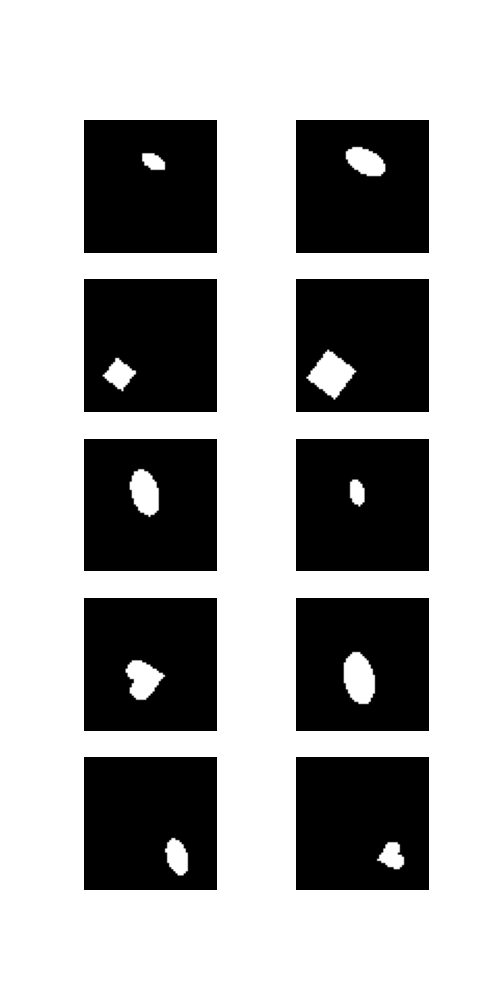
\includegraphics[width=0.7\textwidth]{img/datasets/paired_dsprites}
        \caption{Visualizing Paired dSprites dataset elements}
        \label{fig:paired_dsprites}
    \end{figure}

    \subsection{Scene-dsprites dataset}

    This dataset was created to test the model's ability to reconstruct
    a scene from the sum of object vectors.
    Dataset consists of 2 to 5 non-overlapping figures from dSprites dataset.
    An example of such images on \autoref{fig:scene_dsprites}. This version differs from
    the original multi-dsprites dataset in that the figures do not overlap
    and have the same color.

    \begin{figure}[ht]
        \centering
        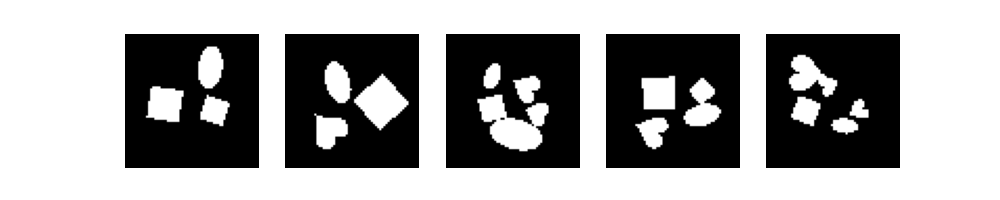
\includegraphics[width=0.7\textwidth]{img/datasets/scene-dsprites}
        \caption{Example of collected scenes in the scene-dsprites dataset}
        \label{fig:scene_dsprites}
    \end{figure}

    \subsection{Paired-Scene-dSprites dataset}

    This dataset combines the capabilities of the first and second dataset.
    There are two objects in the scene image.
    One of these objects can change one feature. \autoref{fig:paired_scene_dsprites}

    \begin{figure}[ht]
        \centering
        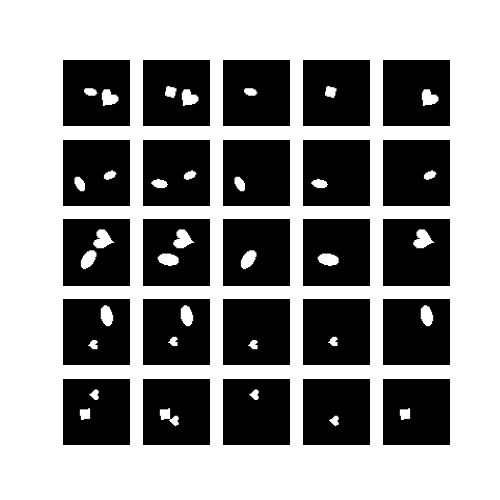
\includegraphics[width=0.6\textwidth]{img/datasets/paired-scenes-dsprites}
        \caption{Example of images from paired-scene-dsprites dataset. From left to right,
            first scene, pair scene, the object to be changed, his pair, second object}
        \label{fig:paired_scene_dsprites}
    \end{figure}


    \section{Models}

    The stages of the work involve successive complications of the model.
    The first stage is that the model will be able to reconstruct the
    original scene from the sum of features (\autoref{fig:sum_features_to_scene}).
    The second stage - the model will be able to reconstruct the scene
    from the sum of objects (\autoref{fig:sum_objects_to_scene}). The third stage - combination of the first
    two approaches - the model should reconstruct the scene
    from the sum of objects, which are represented by the sum of features.

    A VAE is chosen as the basic model. The encoder and
    decoder consist of 4 convolutional and 2 linear layers. The latent
    representation of one figure in dsprites consists of five 1024
    dimensional vectors. One for each feature (\autoref{fig:basic_model}).


    \begin{figure}[ht]{\linewidth}
        \begin{minipage}[b]{0.48\textwidth}
            \centering
            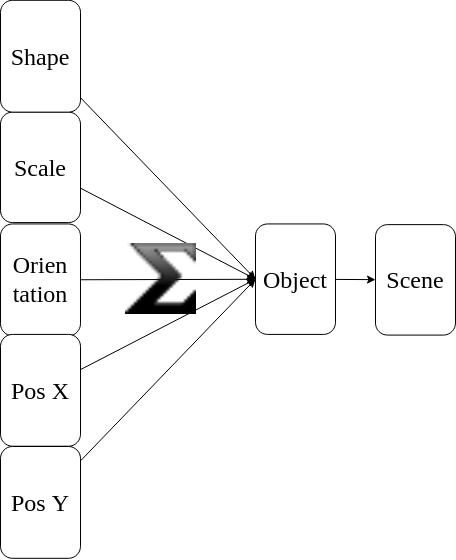
\includegraphics[width=0.7\textwidth]{img/model/sum_features_to_scene}
            \caption{The summation of image features to obtain a latent representation of the object on the scene.}
            \label{fig:sum_features_to_scene}
        \end{minipage}\hfill
        \begin{minipage}[b]{0.48\textwidth}
            \centering
            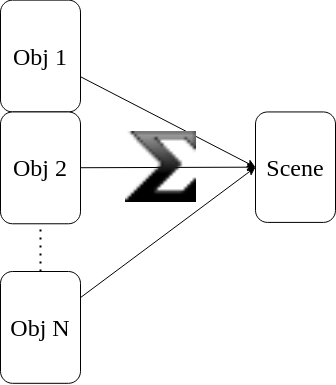
\includegraphics[width=0.7\textwidth]{img/model/sum_objects_to_scene}
            \caption{The summation of image features to obtain a latent representation of the object on the scene.}
            \label{fig:sum_objects_to_scene}
        \end{minipage}
    \end{figure}

    \begin{figure}[ht]
        \centering
        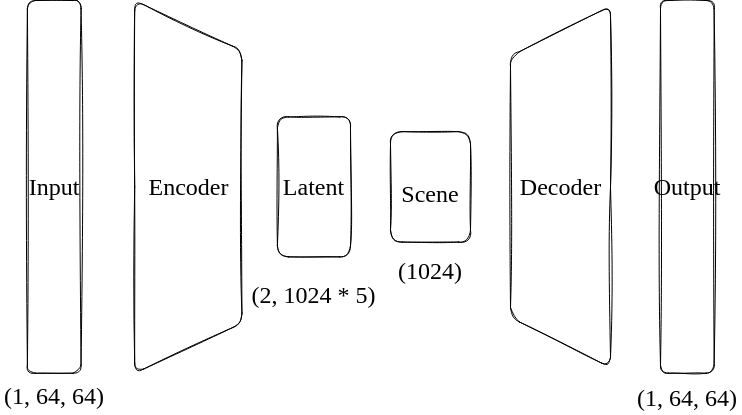
\includegraphics[width=0.6\linewidth]{img/model/basic_model}
        \caption{Diagram of the basic model}
        \label{fig:basic_model}

    \end{figure}

    \subsection{Paired-dSprites model}
    This model reconstructs the scene from the sum of feature vectors.
    The main difficulty is that the vectors representing the features carry
    information only about this feature, as well as that the sum of these
    vectors is reconstructed correctly. Ideally, you want to arrive at a
    model that can assemble a single object with the desired properties
    from different attributes of several objects.

    In order for the model to learn the matching of a particular latent vector
    with an appropriate feature, the following training method is proposed.
    Two images that differ by a single feature are fed to the input of the
    model, and then both images are passed through the encoder, obtaining
    a latent representation.

    We want the four vectors of latent representation corresponding to the
    four features to be independent of the changing feature. Therefore it
    is assumed that one of the vectors encodes the difference between the
    images. To teach this to the model, we swap these difference vectors
    between the input features and try to reconstruct the original images
    crosswise (\autoref{fig:paired_dsprites_model}).


    \begin{figure}[ht]
        \centering
        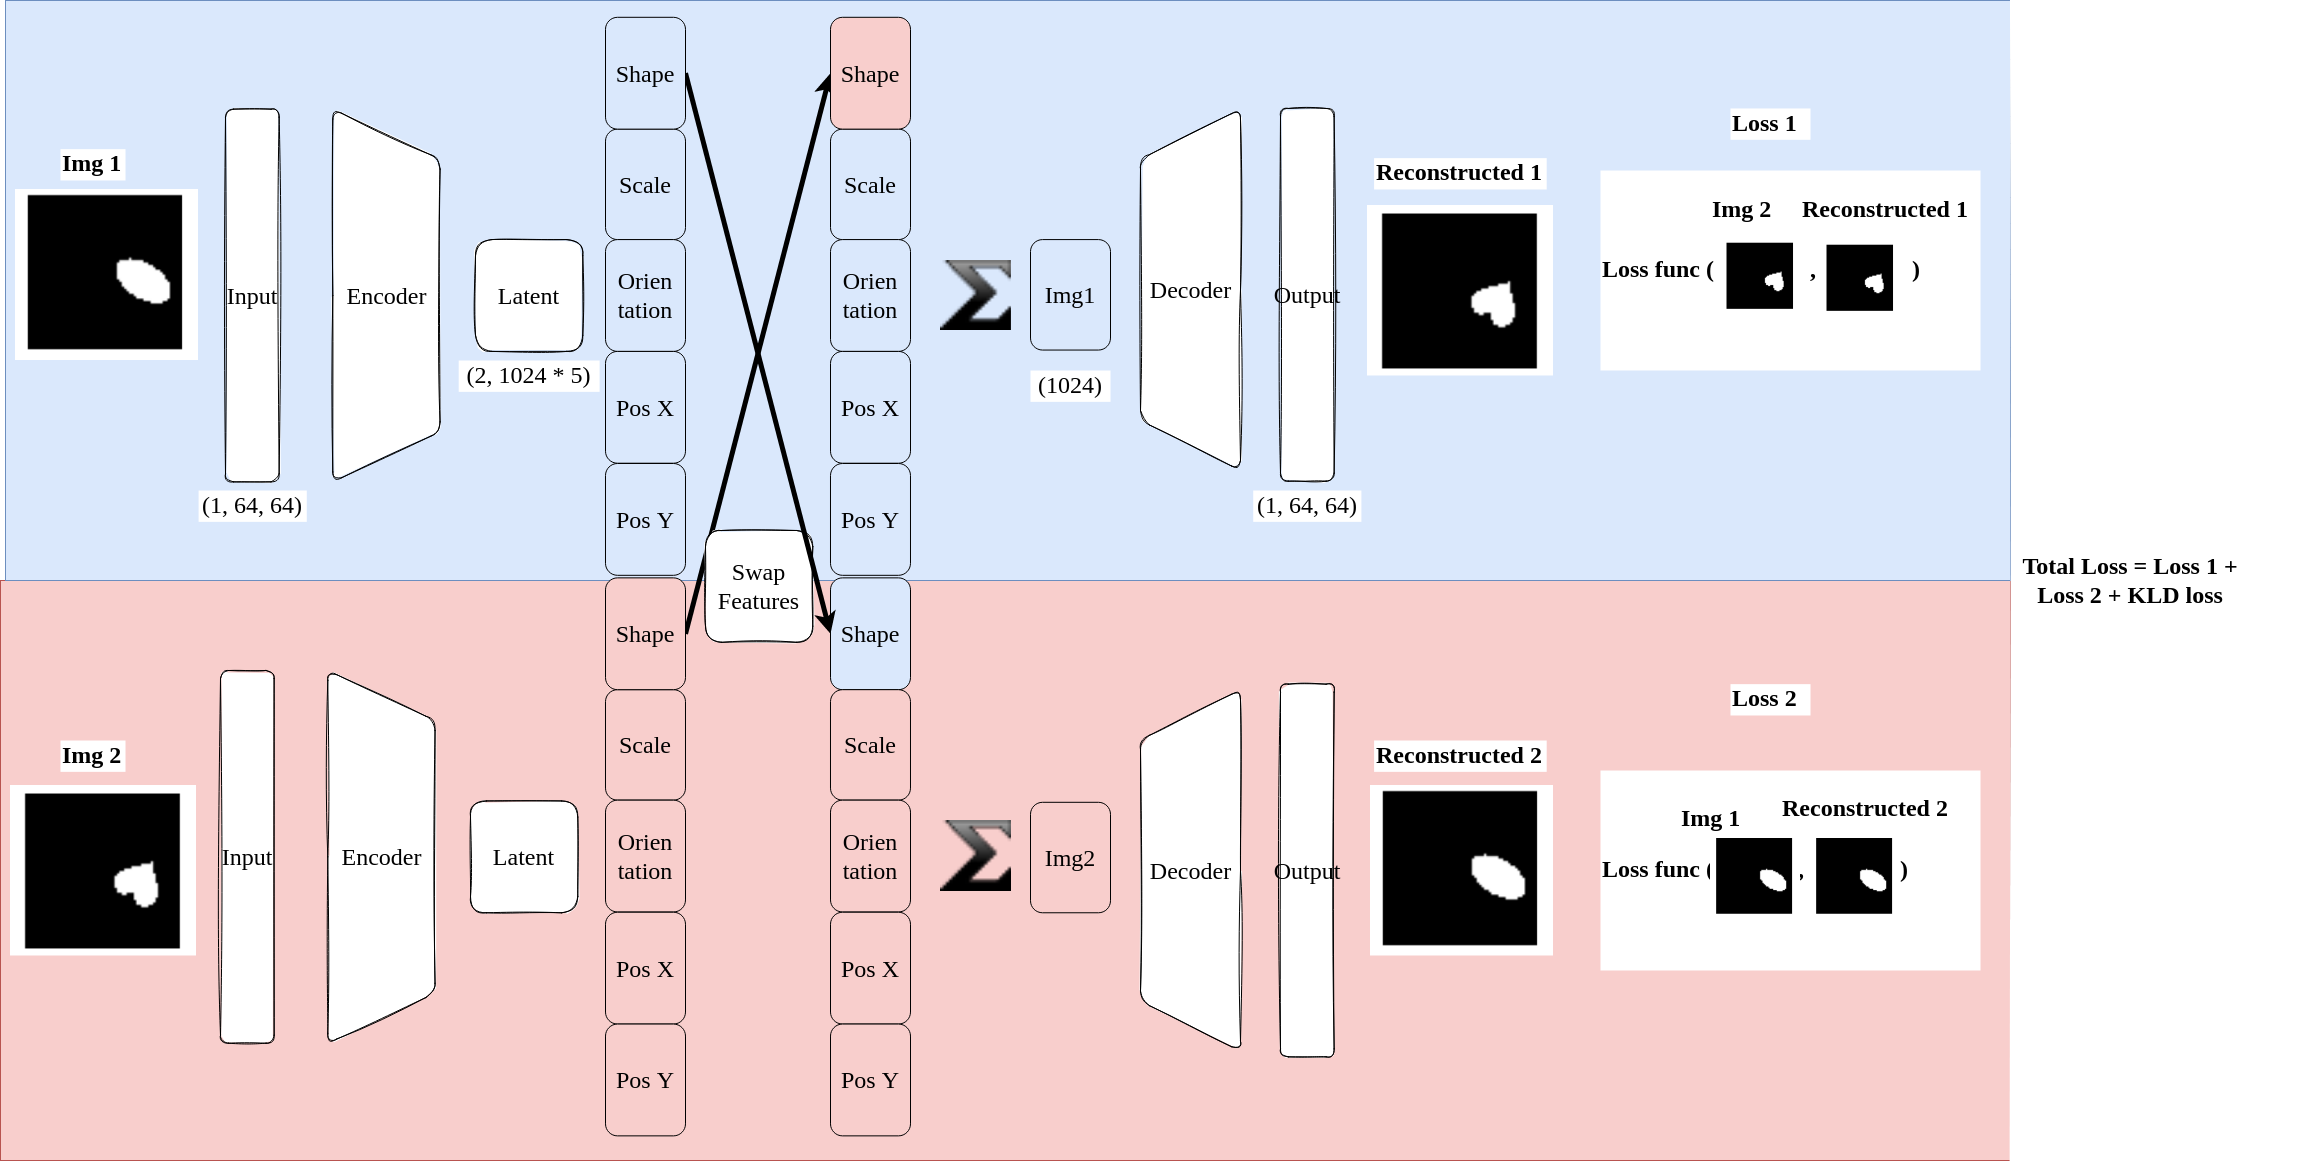
\includegraphics[width=\linewidth]{img/model/paired_dsprites_model}
        \caption{Diagram of the basic model}
        \label{fig:paired_dsprites_model}

    \end{figure}

    \subsection{Scene-dSprites model}

    In the case of scene reconstruction, we take several images from the dataset
    dsprites, pass each image through the encoder and summarize the resulting
    latent representations of objects.

    \subsection{Paired-Scene-dSprites model}
    When combining approaches, we reconstruct the scene from a sum of objects,
    each of which consists of a sum of features. When we successfully partition
    the features into vectors, the problem arises of attributing a particular
    feature to a particular object.

    To solve this problem, we start an item memory, where each property vector
    and each object vector corresponds to its own vector.
    item memory consists of 7 real vectors of the same dimensionality as the
    latent vectors - 1024.
    Vectors are fixed and do not change during training.
    Then during summation we multiply the vectors from the memory by the corresponding
    vectors of the latent representation.


    \section{Results}


    \section{Experiments}

    \begin{tabular}{SSSSSSSS}
        \toprule
        {n} & {Model} & {Image loss} & {Reduction} & {KLD coef} & {Cosine loss} & Quality \\ \midrule
        1   & PD      & MSE          & sum         & 1.0        & 0.0           & Bad     \\
        2   & PD      & MSE          & sum         & 1.0        & 1.0           & Bad     \\
        \midrule
        3   & PD      & MSE          & mean        & 1.0        & 0.0           & Bad     \\
        4   & PD      & MSE          & mean        & 0.1        & 0.0           & Bad     \\
        5   & PD      & MSE          & mean        & 0.01       & 0.0           & Bad     \\
        6   & PD      & MSE          & mean        & 0.001      & 0.0           & Bad     \\
        \midrule
        7   & PD      & MSE          & mean        & 1.0        & 1.0           & Bad     \\
        8   & PD      & MSE          & mean        & 0.1        & 1.0           & Bad     \\
        9   & PD      & MSE          & mean        & 0.01       & 1.0           & Bad     \\
        10  & PD      & MSE          & mean        & 0.001      & 1.0           & Bad     \\
        \midrule
        11  & PD      & BCE          & sum         & 1.0        & 0.0           & Bad     \\
        12  & PD      & BCE          & sum         & 1.0        & 1.0           & Bad     \\
        13  & PD      & BCE          & sum         & 0.1        & 1.0           & Bad     \\
        14  & PD      & BCE          & sum         & 0.0        & 1.0           & Good    \\
        15  & PD      & BCE          & sum         & 0.01       & 1.0           & Good    \\
        \midrule
        16  & PSD     & BCE          & sum         & 0.01       & 1.0           & Good    \\
        17  & PSD     & BCE          & sum         & 0.001      & 1.0           & Bad    \\

        \bottomrule
    \end{tabular}

\end{document}
